\documentclass[12pt,a4paper,oneside]{article}

\usepackage[italian]{babel}
\usepackage[T1]{fontenc}
\usepackage[utf8]{inputenc}
\usepackage[margin=1in]{geometry}
\usepackage{graphicx}
\usepackage{wrapfig}
\usepackage{amsmath}
\usepackage{amssymb}
\usepackage{hyperref}

\usepackage[
	linesnumbered,
	ruled,
	italiano
]{algorithm2e}

\usepackage{tikz}
\usetikzlibrary{arrows,shapes,automata,petri,positioning,calc}

\tikzset{
	place/.style={
		circle,
		thick,
		draw=black,
		fill=gray!50,
		minimum size=6mm,
	},
	state/.style={
		circle,
		thick,
		draw=blue!75,
		fill=blue!20,
		minimum size=6mm,
	},
}

% infinite loop pseudocode command
\SetKwFor{Loop}{Loop forever}{}{EndLoop}

\begin{document}
	
	\title{Secondo assignment programmazione concorrente e distribuita}
	\author{Filippo Barbari, Filippo Benvenuti}
	\date{}%no date
	\maketitle
	
	\tableofcontents
	\newpage
	
	\section{Task programming}
	\subsection{Analisi}
	\subsubsection{Descrizione della simulazione}
	Questa simulazione è una variante della nota "simulazione di $N$ corpi". La simulazione è composta da:
	\begin{itemize}
		\item un numero $N$ di corpi ciascuno dotato di massa ma incorporeo: i corpi non possono colpire nulla tranne i limiti della simulazione
		\item un dominio bidimensionale finito di forma rettangolare e allineato con gli assi cartesiani
		\item una forza repulsiva tra i corpi pari a $F_{ij}=K_{rep}\cdot\dfrac{m_i}{d_{ij}^2}$
		\item una forza d'attrito applicata sui singoli corpi pari a $FR_i=-K_{fri}\cdot{v_i}$
	\end{itemize}
	
	\subsubsection{Analisi dell'algoritmo}
	L'algoritmo seriale è piuttosto semplice. Il corpo di ogni iterazione della simulazione è diviso in due parti:
	\begin{enumerate}
		\item Il calcolo di tutte le forze repulsive (ciclo alle righe 2-4)
		\item L'aggiornamento dei parametri di ogni corpo, in base alle forze calcolate nel primo loop (ciclo alle righe 5-10)
	\end{enumerate}
	Il costo computazionale è $O(b^2\cdot k)$, in cui $b$ rappresenta il numero di corpi e $k$ il numero di iterazioni da compiere.
	\begin{algorithm}
		\SetAlgorithmName{Algoritmo}{}{}
		\KwIn{\texttt{Bodies}, array dei corpi}
		\KwIn{\texttt{bounds}, i bordi della simulazione}
		\KwIn{\texttt{steps}, numero di iterazioni da calcolare}
		
		\For{\texttt{steps} times}{
			\ForEach{Body $b$ in $B$}{
				\texttt{computeTotalForces($b$)}\;
			}
			\ForEach{Body $b$ in $B$}{
				\texttt{computeAcceleration($b$)}\;
				\texttt{updateVelocity($b$)}\;
				\texttt{updatePosition($b$)}\;
				\texttt{checkAndSolveBoundaryCollisions($b$)}\;
			}
		}
		\caption{N-Bodies simulation}
	\end{algorithm}
	
	\subsubsection{Analisi delle dipendenze tra dati}
	\label{sec:dipendenze}
	Questo algoritmo presenta due dipendenze molto importanti:
	\begin{itemize}
		\item il risultato di una determinata iterazione di indice $i > 0$ dipende dal risultato dell'iterazione di indice $i-1$
		\item il risultato dell'aggiornamento dei parametri di un qualsiasi corpo $b_i$ (accelerazione, velocità e posizione) dipende dal risultato del calcolo di tutte le forze repulsive agenti su $b_i$
	\end{itemize}
	
	\subsection{Design}
	\subsubsection{Mutua esclusione}
	Come emerso dall'analisi dell'algoritmo, non è necessario l'utilizzo di alcun meccanismo di mutua esclusione per evitare letture e scritture concorrenti sui parametri dei singoli corpi. Difatti, è sufficiente \textbf{partizionare} l'array globale dei corpi in tante porzioni quanti sono i thread utilizzati, ognuno dei quali si occuperà di aggiornare solamente i corpi della propria partizione.
	
	\begin{algorithm}
		\SetAlgorithmName{Algoritmo}{}{}
		\KwIn{\texttt{Bodies}, array dei corpi}
		\KwIn{\texttt{bounds}, i bordi della simulazione}
		\KwIn{\texttt{steps}, numero di iterazioni da calcolare}
		\KwIn{\texttt{nth}, numero di thread utilizzati}
		\KwIn{\texttt{tid}, indice del thread in esecuzione}
		
		start = length(\texttt{Bodies}) * \texttt{tid} / \texttt{nth}\;
		end = length(\texttt{Bodies}) * (\texttt{tid} + 1) / \texttt{nth}\;
		\For{\texttt{steps} times}{
			\For{i=start; i<end; i++}{
				\texttt{computeTotalForces(\texttt{Bodies[i]})}\;
			}
			\For{i=start; i<end; i++}{
				\texttt{computeAcceleration(\texttt{Bodies[i]})}\;
				\texttt{updateVelocity(\texttt{Bodies[i]})}\;
				\texttt{updatePosition(\texttt{Bodies[i]})}\;
				\texttt{checkAndSolveBoundaryCollisions(\texttt{Bodies[i]})}\;
			}
		}
		\caption{Partitioning N-Bodies simulation}
		\label{alg:sim-partition}
	\end{algorithm}
	
	\subsubsection{Sincronizzazione}
	Un problema più importante consiste, invece, nella \textbf{sincronizzazione} dei thread al fine di non violare nessuna delle due dipendenze tra dati individuate. Non \'e idiomatico utilizzare una Barrier con gli \texttt{ExecutorService} di Java, per cui abbiamo implicitamente sincronizzato i vari \textit{worker} raccogliendo le \texttt{Future} di ogni task e aspettando il loro completamento prima di procedere.
	
	\begin{algorithm}
		\SetAlgorithmName{Algoritmo}{}{}
		\KwIn{\texttt{nth}, numero di thread utilizzati}
		\KwIn{\texttt{tid}, indice del thread in esecuzione}
		
		start = length(\texttt{Bodies}) * \texttt{tid} / \texttt{nth}\;
		end = length(\texttt{Bodies}) * (\texttt{tid} + 1) / \texttt{nth}\;
		\For{\texttt{steps} times}{
			\For{i=start; i<end; i++}{
				\texttt{computeTotalForces(\texttt{Bodies[i]})}\;
			}
			\texttt{barrier()}\;
			\For{i=start; i<end; i++}{
				\texttt{computeAcceleration(\texttt{Bodies[i]})}\;
				\texttt{updateVelocity(\texttt{Bodies[i]})}\;
				\texttt{updatePosition(\texttt{Bodies[i]})}\;
				\texttt{checkAndSolveBoundaryCollisions(\texttt{Bodies[i]})}\;
			}
			\texttt{barrier()}\;
		}
		\caption{Parallel N-Bodies simulation}
		\label{alg:sim-barrier}
	\end{algorithm}

	\subsubsection{GUI}
	Per evitare un eccessivo overhead della GUI, ho scelto di renderla completamente asincrona rispetto alla simulazione.
	
	\subsection{Valutazione}
	\subsubsection{Correttezza}
	\begin{minipage}{.55\textwidth}
		Per semplificare la modellazione dell'algoritmo e la valutazione della correttezza, lavoreremo su una versione semplificata dell'algoritmo \ref{alg:sim-barrier} qui riportata. L'istruzione CF rappresenta il calcolo di \texttt{computeTotalForces}, l'istruzione UP rappresenta un raggruppamento delle istruzioni alle righe 9-12 nell'algoritmo \ref{alg:sim-barrier}. Le istruzioni B1 e B2 rappresentano le barriere di sincronizzazione globale rispettivamente alle righe 7 e 14 dell'algoritmo \ref{alg:sim-barrier}.
	\end{minipage}
	\hfill
	\begin{minipage}{.4\textwidth}
		\begin{algorithm}[H]
			\SetAlgorithmName{Algoritmo}{}{}
			\Loop{}{
				ComputeForces\\
				B1\\
				UpdateParameters\\
				B2
			}
			\caption{Simplified N-Bodies simulation}
		\end{algorithm}
	\end{minipage}
	\hfill
	
	\subsubsection{Java Path Finder}
	Un'analisi, mediante JPF, sul codice realizzato ha rilevato alcune race condition all'interno della classe \texttt{nbodies.sim.data.SimulationData}. In particolare, tali race condition riguardavano il numero dell'iterazione corrente e il tempo di esecuzione misurato, entrambe risolte mediante l'estrazione dei monitor \texttt{Timer} e \texttt{Iteration} all'interno dello stesso package. Infine, JPF non ha rilevato situazioni di \textit{deadlock}.
	
	\subsubsection{Rete di Petri}
	Riporto qui sotto la rete di Petri corrispondente
	Come possiamo notare dal marking graph, la rete di Petri è \textit{bounded}. Le proprietà LTL che si possono esprimere su di esso corrispondono alle due dipendenze tra dati evidenziate nella sezione \ref{sec:dipendenze}. Formalmente:
	\begin{itemize}
		\item $\square ((CF1 \vee CF2) \implies \lozenge B1)$
		\item $\square ((UP1 \vee UP2) \implies \lozenge B2)$
	\end{itemize}

	\begin{center}
		\begin{minipage}{.45\textwidth}
		\scalebox{.7}{
			\begin{tikzpicture}[>=stealth, bend angle=90, auto]
				
				\tikzstyle{transition}=[rectangle,thick,draw=black!75,fill=black!20,minimum size=4mm]
				
				\node [place, tokens=1] (p1) {};
				\node [place] (p2) [node distance=1.5cm, below =of p1] {};
				\node [place] (p3) [node distance=2cm, below =of p2] {};
				\node [place] (p4) [node distance=1.5cm, below =of p3] {};
				
				\node [place, tokens=1] (q1) [node distance=3cm, right of=p1] {};
				\node [place] (q2) [node distance=1.5cm, below =of q1] {};
				\node [place] (q3) [node distance=2cm, below =of q2] {};
				\node [place] (q4) [node distance=1.5cm, below =of q3] {};
				
				\node [place, tokens=1] (n1) [node distance=3cm, right of=q1] {};
				\node [place] (n2) [node distance=1.5cm, below =of n1] {};
				\node [place] (n3) [node distance=2cm, below =of n2] {};
				\node [place] (n4) [node distance=1.5cm, below =of n3] {};
				
				\node [transition] (CF1) [node distance=0.5cm, below =of p1] {CF1} edge [pre] (p1) edge [post] (p2);
				\node [transition] (CF2) [node distance=0.5cm, below =of q1] {CF2} edge [pre] (q1) edge [post] (q2);
				\node [transition] (CFN) [node distance=0.5cm, below =of n1] {CF$n$} edge [pre] (n1) edge [post] (n2);
				\node [transition] (B1) [below =of q2] {B1} edge [pre] (p2) edge [pre] (q2) edge [pre] (n2) edge [post] (p3) edge [post] (q3) edge [post] (n3);
				\node [transition] (UP1) [node distance=0.5cm, below =of p3] {UP1} edge [pre] (p3) edge [post] (p4);
				\node [transition] (UP2) [node distance=0.5cm, below =of q3] {UP2} edge [pre] (q3) edge [post] (q4);
				\node [transition] (UPN) [node distance=0.5cm, below =of n3] {UP$n$} edge [pre] (n3) edge [post] (n4);
				\node [transition] (B2) [below =of q4] {B2} edge [pre] (p4) edge [pre] (q4) edge [pre] (n4) edge [post, bend left] (p1) edge [post, bend right=45] (q1) edge [post, bend right] (n1);
			\end{tikzpicture}}
		\end{minipage}
			\hfill
		\begin{minipage}{.45\textwidth}
			\scalebox{0.7}{
			\begin{tikzpicture}[node distance=1.5cm, >=stealth, bend angle=90, auto]
				% nodes
				\node [place] (M1) {M1};
				\coordinate[left of=M1] (left-M1);
				\coordinate[right of=M1] (right-M1);
				\node [place] (M2) [below =of left-M1] {M2};
				\coordinate[right of=M2] (right-M2);
				\node [place] (M3) [below =of right-M1] {M3};
				\node [place] (M4) [below =of right-M2] {M4};
				\node [place] (M5) [below =of M4] {M5};
				\coordinate[left of=M5] (left-M5);
				\coordinate[right of=M5] (right-M5);
				\node [place] (M6) [below =of left-M5] {M6};
				\coordinate[right of=M6] (right-M6);
				\node [place] (M7) [below =of right-M5] {M7};
				\node [place] (M8) [below =of right-M6] {M8};
				
				%arcs
				\path[->] (M1) edge node {CF1} (M2);
				\path[->] (M1) edge node {CF2} (M3);
				\path[->] (M2) edge node {CF2} (M4);
				\path[->] (M3) edge node {CF1} (M4);
				\path[->] (M4) edge node {B1} (M5);
				\path[->] (M5) edge node {UP1} (M6);
				\path[->] (M5) edge node {UP2} (M7);
				\path[->] (M6) edge node {UP2} (M8);
				\path[->] (M7) edge node {UP1} (M8);
				\path[->] (M8) edge [bend left] node {B2} (M1);
			\end{tikzpicture}}
		\end{minipage}
	\end{center}
	
	\subsection{Prestazioni}
	\subsubsection{Tempi di esecuzione}
	I tempi riportati di seguito fanno riferimento ad un'esecuzione parallela che utilizza 16 thread.
	\newline
	
	\begin{tabular}{|l|l|l|}
		\hline
		\multicolumn{1}{|c|}{\textbf{N. corpi}} & \multicolumn{1}{c|}{\textbf{N. step}} & \multicolumn{1}{c|}{\textbf{Tempo}} \\ \hline
		100 & 1000 & 0,229 \\ \hline
		100 & 10000 & 1,205 \\ \hline
		100 & 50000 & 5,572 \\ \hline
		1000 & 1000 & 1,331 \\ \hline
		1000 & 10000 & 14,95 \\ \hline
		1000 & 50000 & 82,573 \\ \hline
		5000 & 1000 & 33,799 \\ \hline
		5000 & 10000 & 340,124 \\ \hline
		5000 & 50000 & 1704,346 \\ \hline
	\end{tabular}

	\subsubsection{Speedup e Strong scaling efficiency}
	I valori di speedup ed efficienza riportati di seguito sono stati misurati con 1000 corpi e 10000 step. Come si pu\'o notare, la simulazione raggiunge l'apice delle prestazioni con solo 5 thread, ci\'o \'e dovuto all'esigente overhead dell'\texttt{ExecutorService}.
	
	\hfill
	\begin{minipage}{.45\textwidth}
		\centering
		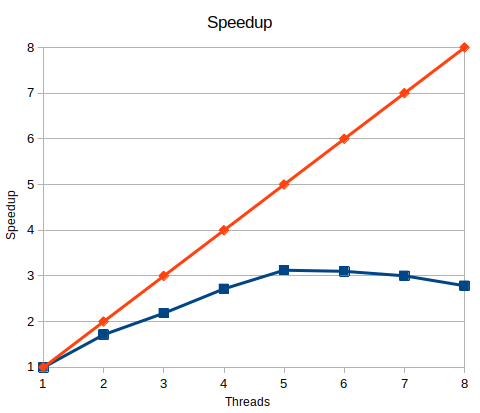
\includegraphics[width=\linewidth]{speedup-no-gui}
		\label{fig:speedup-no-gui}
	\end{minipage}
	\hfill
	\begin{minipage}{.45\textwidth}
		\centering
		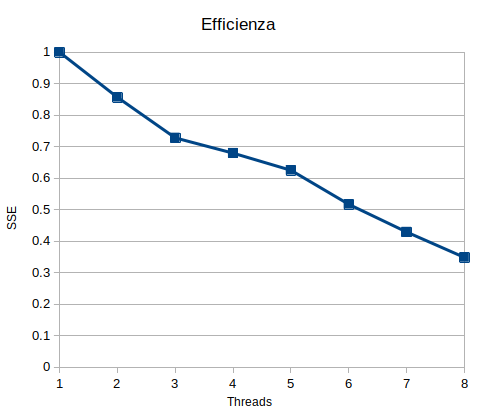
\includegraphics[width=\linewidth]{sse-no-gui}
		\label{fig:sse-no-gui}
	\end{minipage}
	\hfill
	
	\section{Event-driven programming}
	\subsection{Analisi}
	Scopo di questa parte dell'assignment \'e l'implementazione di una libreria asincrona in grado di effettuare il \emph{parsing} di file sorgente Java mediante l'utilizzo dell'\emph{event loop} fornito da \href{https://vertx.io/}{Vert.x}. Abbiamo utilizzato la libreria \href{https://javaparser.org/}{Java Parser} per la fase di parsing.
	
	\subsection{Design}
	Abbiamo realizzato i seguenti eventi, visibili all'interno di \texttt{parser.ProjectElement}, che rappresentano il momento in cui:
	\begin{itemize}
		\item \texttt{packages}: viene trovato un package
		\item \texttt{classes}: viene trovata la dichiarazione di una classe
		\item \texttt{interfaces}: viene trovata la dichiarazione di un'interfaccia
		\item \texttt{fields}: viene trovata la dichiarazione di un campo all'interno di una classe
		\item \texttt{methods}: viene trovata la dichiarazione di un metodo all'interno di una classe
		\item \texttt{methodSignatures}: viene trovata la dichiarazione di un metodo all'interno di un'interfaccia
	\end{itemize}
	Qualsiasi altro costrutto di Java, come Enum o classi innestate, \'e ignorato.
	
	\subsection{Dettagli implementativi}
	Per fermare la computazione in qualunque momento, abbiamo scelto di rilasciare forzatamente le risorse utilizzate da \texttt{vert.x} mediante il metodo \texttt{close()}.
	
	\section{Reactive programming}
	\subsection{Analisi}
	\subsection{Design}
	\subsection{Implementazione}
\end{document}